Software Development Life Cycle (SDLC) is a way to systematically approach software development.
It provides a methodology to improve quality of the desired product and the general work progress. 
Depending on the customer or end users and how clear the project's requirements are different approaches are needed. 
Among the different SDLC methods are the most common ones the older traditional ''Waterfall model'' and the newer ''Iterative model''. \cite{SDLC-Toolsqa}


This chapter will first briefly present the ''waterfall model'' and the ''iterative model'', as well as the argument for choosing the ''iterative model''.
Hereafter, the chapter will contain a description of each iteration throughout the project.


\section{Waterfall model}
This section is based upon \cite{Waterfall-Toolsqa}.
%smid bogens titel ind

The principle of the waterfall model is that the software development process is divided into separate phases, which makes it a sequential design process.
Here the output, in form of documentation, of one phase serves as the input for the next one which means that no phase will start without the previous one being complete.
This is often illustrated as a downward going flow, see \cref{fig:Waterfall}, which is also the reason for its name.

\begin{figure}[H]
	\centering
	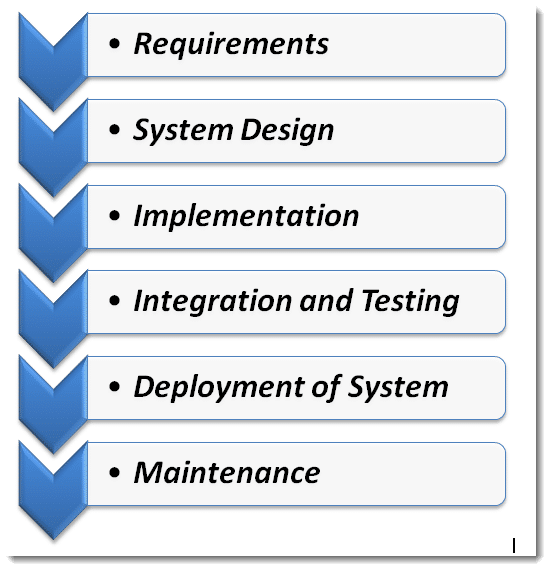
\includegraphics[width=0.4\textwidth]{billeder/WaterFall-Model.png}
	\caption{The Waterfall Model \cite{Waterfall-Toolsqa}.}\label{fig:Waterfall}
\end{figure}

\paragraph{The main benefits} of this model, is that it allows for departmentalization, which makes it possible for a completely different team to work at eg. Implementation compared to the system design part of the project since only the documentation from the system design is necessary to do the implementation.
%andet forslag til formulering: which makes it possible for seperate teams to work at each phase without ever communicating with one another.
Another benefit of this system is how it is easy to manage since there are clear guidelines of what is needed before one phase is done and another can begin.

\paragraph{The main disadvantage} is on the other hand that because of this rigidity it becomes more difficult after every finished phase to go back and change things, when mistakes or misunderstandings of the concept has been made.
Therefore it is also not a beneficial to use when there is a moderate to high risk that the requirements of the system change.
%ville måske være bedre med en simpel textbf for at undgå ekstra mellemrum i pdfen

Since the system developed in this project is done in cooperation with Ipsen, there is a moderate risk of the requirements changing.
This based on the risk of concept misunderstandings, since Ipsen is an expert in her field who has taken contact to software developers with no expertise in this field.
%ikke helt sikker på om jeg forstår this based delen af denne her sætning

\section{Iterative design process} \label{sec:iterativ}
\todo[inline]{Anna: still missing to review this section and add some extra thoughts}
This section is based on \cite{InteractionDesign}.
%vil igen argumentere for at der skal titel på
%virker umiddelbart underligt at have main benefits og disadvatages i egen sektion i den ene men som brødtekst i den anden

The benefit of working iteratively is to continually talk with the users and discuss their needs and wants, determine or redetermine requirements and design a system which gets refined along the way. This ongoing communication with the users and their needs is likewise the center of user-centered approach where there’s a focus on the user’s tasks, empirical measurement and iterative design.
%måske få tydeligere frem at det er nemmere at opdage fejlene tidligere

There are four basic activities when working interaction design which are;
%interaction design har ikke været nævnt før nu?
\textit{establishing requirements, designing alternatives, prototyping,} and \textit{evaluating}. To be able to design a system with the user’s needs and wants in mind it is imperative to know the target users and which activities the system needs to support. This is done through establishing requirements where information of the target users is gathered through data gathering and analysis. When the requirements are settled it is possible to design alternatives ideas that meet these requirements are suggested. Here a conceptual design is formed which describes an abstract outline of how the users can interact with it. Concrete designs infers to the details of the design; which could include colors, sounds, images etc. 

When the design alternative phase is complete a prototype can be developed. The purpose of the prototype is to evaluate with the users whether the criteria has been met and give them an idea of how the system could potentially turn out. The prototype doesn’t necessarily have to consist of a working piece of software; the prototype could also be paper-based in the early stages of the design process. When the prototype is complete then it can be measured an evaluated. The evaluation phase determines whether or not the design is usable and/or acceptable. 

\subsubsection{A simple lifecycle model}
All of the before-mentioned activities are related in an iterative design process. This is shown visually in \cref{fig:LifecycleModel}. The lifecycle model is a simplified version of reality and isn’t meant to be prescriptive, and depending on the project it isn’t always possible to go through all of the phases described. 
%Anna:synes ikke denne tekst passer ind
%Though the model is developed through Sharp, Rogers and Preece’s research of how software engineering is practiced in the field. 

\begin{figure}[h]
	\centering
	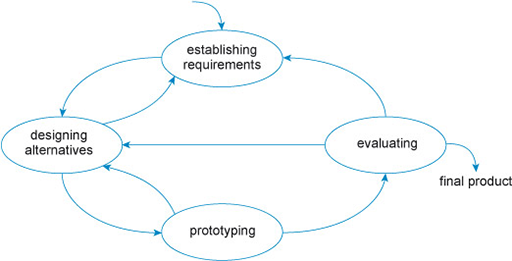
\includegraphics[width=0.75\textwidth]{billeder/lifecycle.png}
	\caption{Lifecycle model \citep[p.~332]{InteractionDesign}}\label{fig:LifecycleModel}
\end{figure}

According to Sharp, Rogers and Preece “Most projects start with establishing requirements” \citep[p.~333]{InteractionDesign}. It is from this first activity that it’s possible to go into the ‘designing alternatives’ activity from where a prototype in the ‘prototyping’ activity, can be developed which in turn can be evaluated by the users in the ‘evaluating’ activity. From this evaluation the designers can specify new or redefined requirements, or they can go directly to redesign or deem the project done.
% Henrik: Måske brug noget af nedenstående tekst som introduktion til "den iterative ..." afsnit? :-)
\subsubsection{Using of the lifecycle model in the project}
Throughout the project it is intended to design a system iteratively with a specific user’s needs and wants integrated into the designs and tests. This is the basis of choosing to work with the lifecycle model as a model to reflect over which activity is being used throughout the stages of the project. The lifecycle model is likewise a good indicator of when an iteration is done and when a new one has been commenced.




